\documentclass{jhwhw}
\usepackage{amsmath}
\usepackage{amssymb}
\usepackage{tikz}
\usepackage[makeroom]{cancel}
\usetikzlibrary{patterns}
\title{MATH 5510: Topology: HW 1}
\author{Markus Foote}

\begin{document}
\problem{}%1
 Let $|u|$ be a norm on $\mathbb{R}^n$ and $d(x,y) = |y - x|$ the corresponding metric. A norm is called \emph{strictly convex} if for any two distinct points $u,v\in S(0,1)$, every interior point of the segment from $u$ to $v$ lies in the open ball $B(0,1)$,  In other words, if $|u|=1, |v| = 1$, $u\ne v$, then for all $s$ with $0<s<1$ we have $|(1-s) u + s v |   <1$.  Give two examples of norms on $\mathbb{R}^2$: one that is strictly convex, and one that is not.

\solution{}
\part{}
$|u| = \sqrt{x_1^2+x_2^2+\cdots+x_n^2}$ is a strictly convex norm. This can be shown by examining the ball $B(0,1)$ and the line segment $\overline{uv}$ between $u=(0,1)$ and $v=(1,0)$. This line lies strictly inside the ball, showing strict convexity.
\begin{center}
	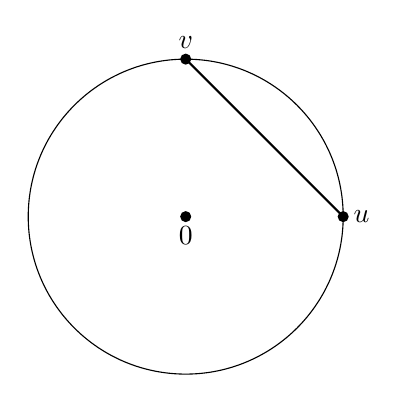
\begin{tikzpicture}
	\fill (0,0) circle[radius=2pt] node[below]{$0$};
	\draw (0,0) circle (2cm);
	\fill (0,2cm) circle[radius=2pt];
	\fill (2cm,0) circle[radius=2pt];
	\draw [thick] (0,2cm) node[above]{$v$}-- (2cm,0)node[right]{$u$};
	\end{tikzpicture}
\end{center}

\part{}
$|u| = |x_1|+|x_2|+\cdots+|x_n|$ is \textbf{not} a strictly convex norm. This can be shown by examining the ball $B(0,1)$ and the line segment $\overline{uv}$ between $u=(0,1)$ and $v=(1,0)$. This line lies on the edge of the ball, showing that strict convexity does not exist for this norm (while regular convexity does).
\begin{center}
	\begin{tikzpicture}
	\fill (0,0) circle[radius=2pt] node[below]{$0$};
	\draw (0,2cm) -- (2cm,0) -- (0,-2cm) --( -2cm,0) -- (0,2cm) ;
	\fill (0,2cm) circle[radius=2pt];
	\fill (2cm,0) circle[radius=2pt];
	\draw [thick] (0,2cm) node[above]{$v$}-- (2cm,0)node[right]{$u$};
	\end{tikzpicture}
\end{center}


\problem{} %2
Suppose $|u|$ is a strictly convex norm. Prove the following:
\begin{enumerate}
	\item If $u\ne 0, v\ne 0$ and $|u + v| = |u| + |v|$, then $v = \lambda u$ for some $\lambda \in \mathbb{R}, \lambda >0$.
	
	\emph{Suggestion}:Let $ u' = u/|u|$ and $v' = v/|v|$. Use the identity
	$$
	u + v = (|u| + |v|) \Big{(} \Big{(}1 - \frac{|v|}{|u| + |v|}\Big{) }u' + \frac{|v|}{|u|+ |v|} v' \Big{)}
	$$
	
	\item If $x,y,z$ satisfy equality in the triangle inequality, that is, $d(x,z) = d(x,y) + d(y,z)$, then $x,y,z$ are co-linear and $y$ lies between $x$ and $z$.
\end{enumerate}

\solution{}

\part{}

Proof by contrapositive: if $|u + v| < |u| + |v|$ then $v \neq \lambda u$ for some $\lambda \in \mathbb{R}, \: \lambda >0$, then:
\begin{gather}
\forall s \in (0,1), \: |(1-s)u + sv| < 1\\
|u + v| = \Big|(|u| + |v|) \Big{(} \Big{(}1 - \frac{|v|}{|u| + |v|}\Big{) }u' + \frac{|v|}{|u|+ |v|} v' \Big{)} \Big|\\
|u+v|< |(|u| + |v|)| \\
|u + v| < |u| + |v|
\end{gather}
so $\to v = \lambda u$.


\part{}
Let $u = x-y$ and $v = y-z$:
\begin{gather}
d(x,z) = |u + v|\\
d(x,y) = |u|\\
d(y,z) = |v|
\end{gather}
From (a) we know $v = \lambda u$, thus the vectors are scaled versions of each other, which means they are in the same direction, thus the endpoints $x,y,z$ are co-linear.
\begin{align}
|u| &< (1+\lambda) |u|\\
d(x,y) &< |u| + \lambda |u|\\
d(x,y) &< |u| + |\lambda u|\\
d(x,y) &< |u| +|v|\\
d(x,y) &< |u+v|\\
d(x,y) &< d(x,z)
\end{align}
thus $y$ is closer to $x$ than $z$ is to $x$ and they are on the same line, so $y$ lies between $x$ and $z$.


\problem{}%3
 Let $X = \{ (x,1):x\in\mathbb{R}\}\subset\mathbb{R}^2$. Let $d$ be the restriction of the French-railway metric, that is, $d(x,y) = d_{FR}(x,y)$ for all $x,y\in X$.  Let $d'(x,y)$ be the restriction of  $d_{(2)}$, that is, $d'(x,y) = d_{(2)}(x,y)$ for all $x,y\in X$.   Let $f:(X,d)\to (X,d')$ be the identity map.

\begin{enumerate}
	\item Is $f$ Lipschitz?
	\item Is $f$ bi-Lipschitz?
	\item Is $f$ a homeomorphism?
\end{enumerate}


\solution{}
\part{}
$f$ is Lipschitz:
\begin{gather}
d'(f(x),f(y)) \le c\: d(x,y)\\
d'(x,y) \le c \: d(x,y)\\
\sqrt{(x_1^2-y_1^2)+(1^2-1^2)} \le c\: \left(\sqrt{x_1^2+1^2}+\sqrt{y_1^2+1^2}\right) \text{ for } x\ne y\\
 \text{or }\:0=0 \text{ for } x= y\\
\sqrt{x_1^2-y_1^2} \le c\: \left(\sqrt{x_1^2+1^2}+\sqrt{y_1^2+1^2}\right)\\
c = 1 
\end{gather}
\part{}
$f$ is not bi-Lipschitz:

$f$ cannot be bi-Lipschitz if its inverse $f^{-1}$ is not Lipschitz. $f^{-1}$ cannot be Lipschitz if it is not continuous:
$f^{-1}:(X,d')\to(X,d)$:
\begin{gather}
\forall x\in X,\forall \varepsilon >0 \:\exists \:\delta (=\delta (x,\varepsilon) )\: s.t.\: d'(x,y) < \delta, \: d(f^{-1}(x),f^{-1}(y)) < \varepsilon \\
\text{Let } \mathbf{x}=(x,1), \mathbf{y}=(y,1),\: x,y>0,\:y>x>\varepsilon>0\\
d(f^{-1}(\mathbf{x}),f^{-1}(\mathbf{y})) =d(\mathbf{x},\mathbf{y})= \sqrt{x^2 +1}+\sqrt{y^2+1}> \sqrt{y^2+1} > \sqrt{y^2} =y>\varepsilon
\end{gather}
thus $f^{-1}$ is not continuous, thus not Lipschitz, thus $f$ is not bi-Lipschitz.


%\begin{gather}
%\forall c_1 \exists x_1,y_1\in \mathbb{R} \: s.t. \: c_1\:\sqrt{x_1^2+1^2}+\sqrt{y_1^2+1^2} \nleq sqrt{(x_1^2-y_1^2)} ,\text{ which is } x_1 = c_1, y_1 = c_1 + 1 
%\end{gather}

\part{}
$f$ is not a homeomorphism because $f^{-1}$ is not continuous, as shown in part (b).


\problem{}%4
 Prove the following: 
 \begin{enumerate}
	\item Any isometry of $(\mathbb{R}^2,d_{(1)})$  to itself sends horizontal lines to horizontal or vertical lines, and vertical lines to horizontal or vertical lines.
	(You may use the fact that an interval is not homeomorphic to a non-degenerate rectangle.)
	
	\item Prove that any isometry of $f:(\mathbb{R}^2,d_{(1)})\to (\mathbb{R}^2,d_{(1)})$ that fixes the origin must be of the form $f((x_1,x_2) )= (\pm x_1,\pm x_2)$ or $f((x_1,x_2)) = (\pm x_2, \pm x_1)$.  (Reduce to: an isometry satisfying $f(x_1,0) = (x_1,0)$ and $f(0,x_2) = (0,x_2)$ is the identity)
\end{enumerate}

\solution{}
\part{}
If $f\: : \: (X,d) \to (Y,d')$ is an isometry, then $f$ takes equality sets to equality sets, $f(E_d(x,y)) = E_d(f(x),f(y))$. We show that the equality sets are not homeomorphic, except when horizontal lines are mapped to horizontal or vertical lines. Similarly, maps which take vertical lines to anything except vertical or horizontal lines are not isometries. The equality sets below are homeomorphic in the second and third diagram, line segments; the equality sets of in the first diagram are not homeomorphic (rectangle to line segment).

\begin{center}
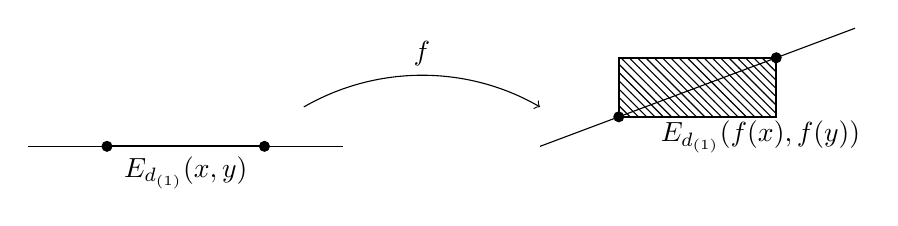
\begin{tikzpicture}
	\draw (-4,0) -- (0,0);
	\fill (-3,0) circle[radius=2pt] coordinate (a);
	\fill (-1,0) circle[radius=2pt] coordinate (b);
	\draw [thick] (a) -- (b) node[midway,below]{$E_{d_{(1)}}(x,y)$};
	\draw [->] (-0.5,0.5) arc (120:60:3) node[midway,above]{$f$} coordinate (n);
	\coordinate (m) at ([yshift=-0.5cm, xshift=-0.0cm]n) ;
	\draw (m) -- ([xshift=4cm,yshift=1.5cm]m) coordinate (p) ;
	\path (m) -- (p) coordinate [midway] (l2) ;
	\path (m) -- (l2) coordinate [midway] (l1) ;
	\path (l2) -- (p) coordinate [midway] (l3) ;
	\fill (l1) circle[radius=2pt] ;
	\fill (l3) circle[radius=2pt] ;
	\draw [pattern=north west lines,thick] (l1) rectangle (l3) node[pos=0.9,below=0.6cm] {$E_{d_{(1)}}(f(x),f(y))$} ;
\end{tikzpicture}
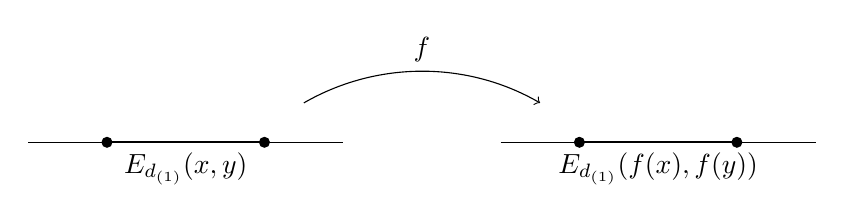
\begin{tikzpicture}
\draw (-4,0) -- (0,0);
\fill (-3,0) circle[radius=2pt] coordinate (a);
\fill (-1,0) circle[radius=2pt] coordinate (b);
\draw [thick] (a) -- (b) node[midway,below]{$E_{d_{(1)}}(x,y)$};
\draw [->] (-0.5,0.5) arc (120:60:3) node[midway,above]{$f$} coordinate (n);
\coordinate (m) at ([yshift=-0.5cm,xshift=-0.5cm]n) ;
\draw (m) -- ([xshift=4cm]m) coordinate (p) ;
\path (m) -- (p) coordinate [midway] (l2) ;
\path (m) -- (l2) coordinate [midway] (l1) ;
\path (l2) -- (p) coordinate [midway] (l3) ;
\fill (l1) circle[radius=2pt] ;
\fill (l3) circle[radius=2pt] ;
\draw [pattern=north west lines,thick] (l1) rectangle (l3) node[pos=0.5,below=] {$E_{d_{(1)}}(f(x),f(y))$} ;
\end{tikzpicture}
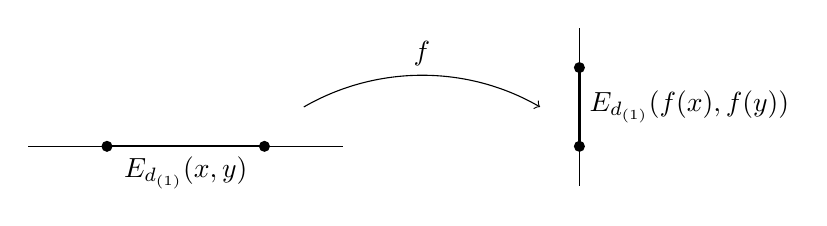
\begin{tikzpicture}
\draw (-4,0) -- (0,0);
\fill (-3,0) circle[radius=2pt] coordinate (a);
\fill (-1,0) circle[radius=2pt] coordinate (b);
\draw [thick] (a) -- (b) node[midway,below]{$E_{d_{(1)}}(x,y)$};
\draw [->] (-0.5,0.5) arc (120:60:3) node[midway,above]{$f$} coordinate (n);
\coordinate (m) at ([yshift=-1cm,xshift=0.5cm]n) ;
\draw (m) -- ([xshift=0cm,yshift=2cm]m) coordinate (p) ;
\path (m) -- (p) coordinate [midway] (l2) ;
\path (m) -- (l2) coordinate [midway] (l1) ;
\path (l2) -- (p) coordinate [midway] (l3) ;
\fill (l1) circle[radius=2pt] ;
\fill (l3) circle[radius=2pt] ;
\draw [pattern=north west lines,thick] (l1) rectangle (l3) node[pos=0.5,right] {$E_{d_{(1)}}(f(x),f(y))$} ;
\end{tikzpicture}
\end{center}

\part{}
Using (a), we can investigate identity cases for a point $(x_1,0)$ or $(0,x_2)$:
\begin{align}
H\to H&: f(x_1,0) \to (ax_1,0) \: \text{for} \: a \in \mathbb{R}\\
H \to V&: f(x_1,0) \to (0,bx_1) \: \text{for} \: b \in \mathbb{R}\\
V \to H&: f(0,x_2) \to (cx_2,0) \: \text{for} \: c \in \mathbb{R}\\
V \to V&: f(0,x_2) \to (0,dx_2) \: \text{for} \: d \in \mathbb{R}
\end{align}
We know that the origin is preserved ,$f((0,0)) \to (0,0)$, and using that $f$ is an isometry, 
\begin{gather}
d_1(f(x_1,0),f(0,0)) = d_1((ax_1,0),(0,0))\\
|x_1|= |ax_1| \\
\implies a = \pm 1
\end{gather}
A similar argument may be constructed for $b$, $c$, and $d$, so $|a|=|b|=|c|=|d|=|1|$. So a point on an axis must be mapped to a point on an axis that is the same $d_{(1)}$ distance from the origin. A similar point on a horizontal or vertical line with distance $k$ from the axis that intersects the line will be mapped to another vertical or horizontal line $k'$:
\begin{equation}
f(x_1,k) \to (\pm x_1,k')
\end{equation}
Then, again as $f$ is an isometry:
\begin{gather}
d_1\big(f(x_1,k),f(x_1,0)\big)=d_1\big((x_1,k),(x_1,0)\big)\\
d_1(( ax_1,k'),(ax_1,0)) \\
|ax_1 - ax_1| + |k' - 0| = |x_1 - x_1| + |k - 0|\\
|k'| = |k|
\end{gather}
therefore as long as $k$ is the same distance above or below (positive or negative) from the axis, the $d_{(1)}$ distance is preserved. So for a point that is along a horizontal or vertical line, that point is still the same distance from the origin. And we know the zero-crossing of the line is the same distance from the origin. This all shows that an isometry  $f:(\mathbb{R}^2,d_{(1)})\to (\mathbb{R}^2,d_{(1)})$ that fixes the origin must be of the form $f((x_1,x_2) )= (\pm x_1,\pm x_2)$ or $f((x_1,x_2)) = (\pm x_2, \pm x_1)$.

\problem{}%5
Let $S^2 = \{x = (x_1,x_2,x_3)\in\mathbb{R}^3 : x_1^2 + x_2^2 + x_3^2  = 1\}$ be the unit sphere  in $\mathbb{R}^3$.  Let $d_i(x,y) = \cos^{-1}(x\cdot y)$, where $x\cdot y$ is the usual dot product of vectors in $\mathbb{R}^3$, be the intrinsic metric on $S^2$ (length of the great circle arc joining $x$ and $y$).    Prove that $d_i$ satisfies the triangle inequality.

\noindent\emph{Suggestion}: Use the fact that for any 3 vectors $x,y,z\in\mathbb{R}^3$ the determinant of the matrix
$$
A = 
\left( \begin{array}{ccccc}
x\cdot x &\ & x\cdot y &\ & x\cdot z \\
y\cdot x &\ & y\cdot y &\ & y\cdot z \\
z\cdot x &\ & z\cdot y &\ & z\cdot z 
\end{array} \right)
$$
is $\ge 0$.   For $x,y,z\in S^2$, apply $\cos$ to both sides of the desired inequality  $\cos^{-1}(x\cdot z) \le \cos^{-1}(x\cdot y) + \cos^{-1}(y\cdot z)$ and reduce the resulting inequality to  $\det(A)\ge 0$.
\solution{}

\begin{gather}
d(x,z)\le d(x,y)+d(y,z)\\
\cos^{-1}(x\cdot z) \le \cos^{-1}(x\cdot y) + \cos^{-1}(y\cdot z)\\
\cos(\cos^{-1}(x\cdot z)) \ge cos(\cos^{-1}(x\cdot y) + \cos^{-1}(y\cdot z))\\
\text{apply } \cos(\alpha+\beta) = \cos(\alpha)\cos(\beta)-\sin(\alpha)\sin(\beta)\\
(x\cdot z) \ge \cos(\cos^{-1}(x\cdot y))\cos(\cos^{-1}(y\cdot z))-\sin(\cos^{-1}(x\cdot y))\sin(\cos^{-1}(y\cdot z))\\
\text{apply } \sin(\cos^{-1}(x)) = \sqrt{ 1 -x^2}\\
(x\cdot z) \ge (x\cdot y)(y\cdot z)-\sqrt{ 1 -(x\cdot y)^2}\sqrt{ 1 -(y\cdot z)^2}\\
\sqrt{ 1 -(x\cdot y)^2}\sqrt{ 1 -(y\cdot z)^2} \ge (x\cdot y)(y\cdot z)-(x\cdot z)\\
\left(\sqrt{ 1 -(x\cdot y)^2}\sqrt{ 1 -(y\cdot z)^2}\right)^2 \ge \left((x\cdot y)(y\cdot z)-(x\cdot z)\right)^2\\
( 1 -(x\cdot y)^2)(1 -(y\cdot z)^2) \ge ((x\cdot y)(y\cdot z))^2-2(x\cdot y)(y\cdot z)(x\cdot z)+(x\cdot z)^2\\
1 -(x\cdot y)^2-(y\cdot z)^2 + \cancel{(x\cdot y)^2(y\cdot z)^2} \ge \cancel{(x\cdot y)^2(y\cdot z)^2}-2(x\cdot y)(y\cdot z)(x\cdot z)+(x\cdot z)^2\\
1 -(x\cdot y)^2-(y\cdot z)^2  \ge -2(x\cdot y)(y\cdot z)(x\cdot z)+(x\cdot z)^2\\
1 -(x\cdot y)^2-(y\cdot z)^2-(x\cdot z)^2 + 2(x\cdot y)(y\cdot z)(x\cdot z) \ge 0\\
1-(z\cdot y)(y\cdot z) - (x\cdot y)(y\cdot x) - (x\cdot z)(z\cdot x) + 2 (x\cdot y)(y\cdot z)(x\cdot z) \ge 0\\
\text{Use } (x\cdot x)=(y\cdot y)=(z\cdot z)=1\\
(x\cdot x)(y\cdot y)(z\cdot z) -(x\cdot x)(z\cdot y)(y\cdot z) - (z\cdot z)(x\cdot y)(y\cdot x)  \qquad\qquad\nonumber\\
\qquad\qquad\qquad -(y\cdot y)(x\cdot z)(z\cdot x) + 2 (x\cdot y)(y\cdot z)(x\cdot z) \ge 0\\
\det(A) \ge 0
\end{gather}


\end{document}